\documentclass[11pt]{article}

\usepackage{amsmath,amssymb}
\usepackage{a4wide}
\usepackage{graphicx}
\usepackage{tikz}



\begin{document}
\section{The algorithms}
\label{se:algorithms}
\subsection{Network Algorithm}
\subsubsection{Outline}
The algorithm consists of the following steps:
\begin{enumerate}
  \item Given the set $P$ create a graph $G(V,E)$ where $V=P$ and $E=V\times V$.
  \item Compute the $EMST$ of $G$.
  \item Compute $EMST_{add}$ by connecting each endpoint, if possible, to a nearby node.
  \item Find segment that divert from straight roads and remove these segments to get $EMST_{rem}$.
  \item Connect
\end{enumerate}
  \begin{figure}[h]
  \centering
      \graphicspath{ {images/}}
      \includegraphics[width=0.7\linewidth]{NetworkMST}
      \label{fig:EMST}
      \caption{$EMST$ for a given set $p$. The red dotted circles indicate the misssing road segments.}
  \end{figure}
\subsubsection{Description}
Given the set $P$ of points in $\mathbb{R}^2$ first the Eucledian minimum spanning tree $EMST$ is calculated by using Prim's algorithm. This results in a connected graph $RN(P,S)$, where $s_{a,b}\in S$ represents a road segment between points $a,b \in P$, that gives a good approximation of the road network but some road segments may be missing.%TODO ref 

From $RN$ a new graph is made in which the missing road segments are added in a naive way. For each point $p_1 \in P$ that has degree $1$ the nearest point $p_n \in Adj_{p_1,5}$ is found such that the angle between the segment that contains $p_n$ and point $p_n$ is $>90$, this avoids that roads contain sharp angles. 

The next step in the algorithm is to find road segments that diverge from straight roads. $\alpha_{straight}$ is defined as the minimum angle for which two consecutive road segments are consider a straight road. $\alpha_{min}$ is the minimum angle that a road segment must make with the previous segment for it not to be a bend. For every point $p_2 \in P$ that has degree $2$ there are two points $r_1, q_1 \in P$ which make up the segments $s_{p_2, q_1}$ and $s_{p_2,r_1}$. Segments $s_{q_1, q_2}$ and $s_{r_1,r_2}$ are the segments that are connected to $q_1$ and $r_1$. $\theta=\varphi(s_{p_2, q_1},s_{p_2,r_1})$, if $\theta> \alpha_{straight}$ then $\alpha_1=\varphi(s_{p_2, q_1},s_{q_1, q_2})$ and $\alpha_2=\varphi(s_{p_2, r_1},s_{r_1, r_2})$. If $\alpha_1$ or $\alpha_2$ $<\alpha_{min}$ then $s_{q_1, q_2}$ or $s_{r_1, r_2}$ is removed from $S$.

\begin{figure}[h]
\centering
  \graphicspath{ {images/}}
  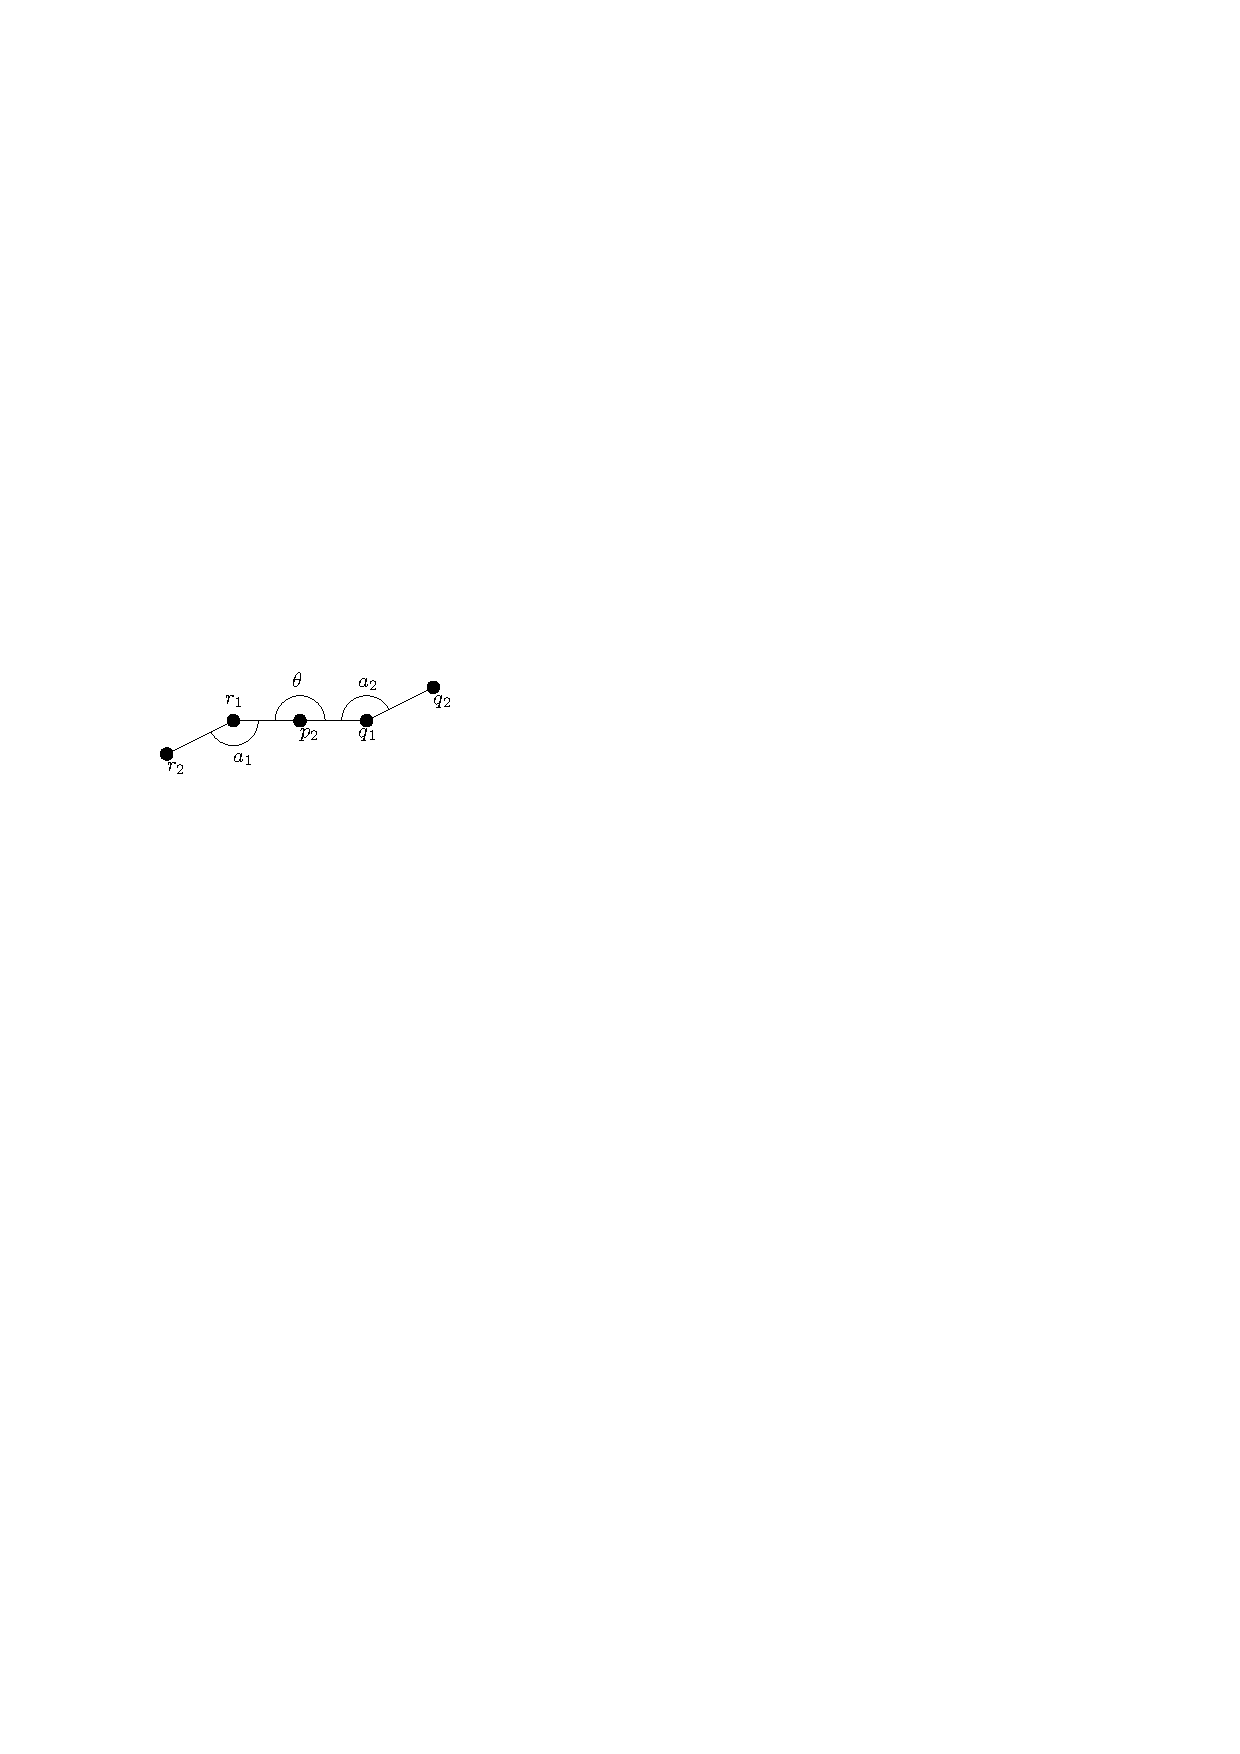
\includegraphics[width=0.9\linewidth]{NetworkRemoveSegmentsDetail}
  \label{fig:NetworkRemove}
  \caption{Calculation of $\theta$, $\alpha_1$ and $\alpha_2$}
\end{figure}
  
$RN$ is now a unconnected graph. For $RN$ to represent the road network it must be connected. Points that are not connected have degree 1. $d_{max}$ is defined as the maximum distance that is allowed between two points for them to form a new segment. For every point $p_3 \in P$ that has degree 1, the 10 most nearest points are found, $q_3 \in P$ is the point such that $s_{q_3, p_3} \in S$. Let $p_{near} \in Adj_{p_3,10}$ be such a point and $\alpha_3=\varphi(s_{q_3, p_3},s_{p_3, p_{near}}$. If $\alpha_3>\alpha_{min}$, $d(p_3,p_{near})<d_{max}$ and $s_{p_3, p_{near}}$ does not intersect any other segment in $S$ then $S=S \cup s_{p_3, p_{near}}$. In case a intersection does occur at point $u_1 \in U$ with segment $s_{w_1, w_2}\in S$, $P_{add}=P_{add}\cup u$. Four new segments $s_{w_1, u_1}$, $s_{u_1, w_2}$, $s_{p_3, u_1}$ and $s_{u_1, p_{near}}$ are added to $S$ and $s_{w_1, w_2}$ is removed from $S$\ref{fig:AddIntersect}.

\begin{figure}[h]
\centering
      \graphicspath{ {images/}}
      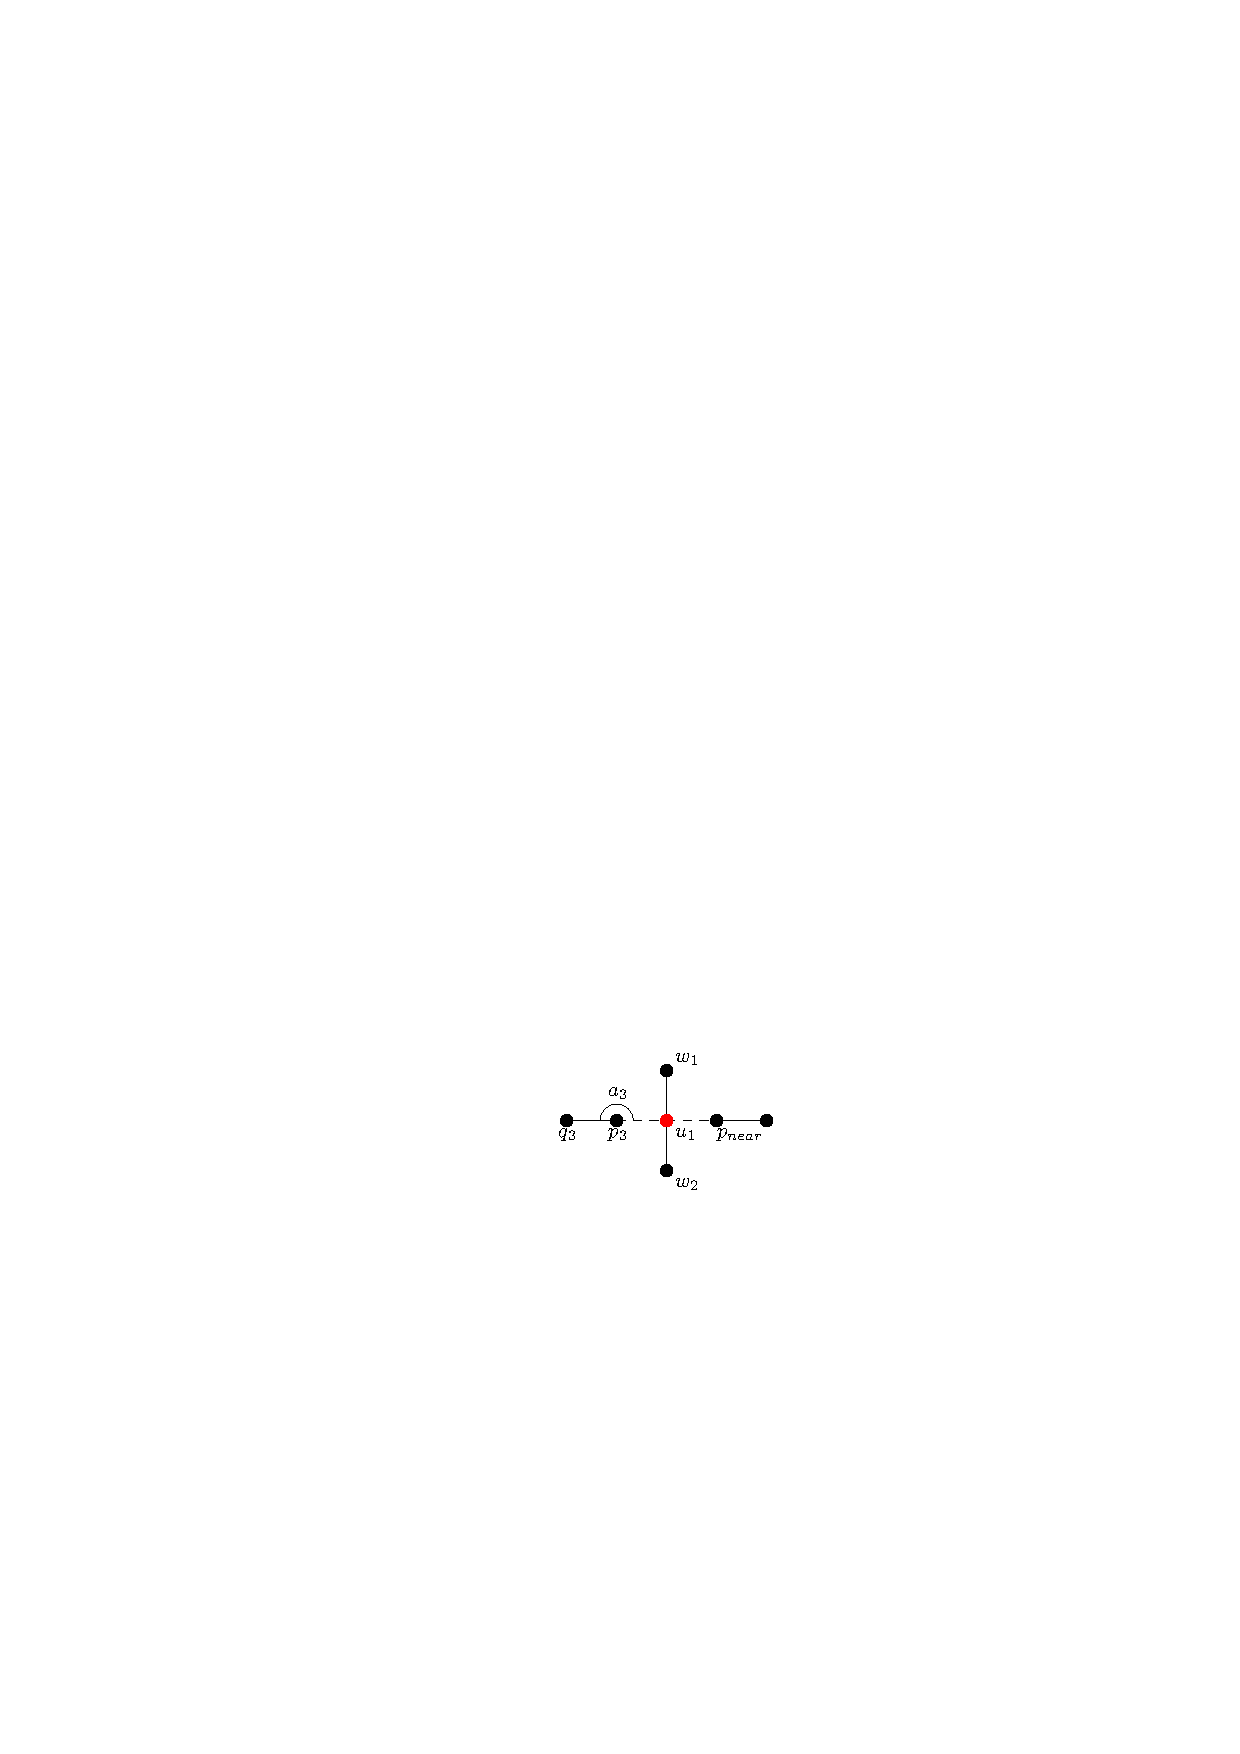
\includegraphics[width=0.9\linewidth]{NetworkAddIntersection}
      \label{fig:AddIntersect}
      \caption{Adding a new segment that intersects the existing segment $s_{w_1,w_2}$}.
  \end{figure}

When no such point is found in $Adj_{p_3,10}$ the segment $s_{q_3, p_3}$ is extended with a new segment $s_{p_3,q_4}$ where $q_4 \in U$ and $d(p_3,q_4)<d_{max}$. If $s_{p_3,q_4}$ intersects with a other segment $s_{w_3,w_4} \in S$ at $u_2 \in U$ then three new segments $s_{p_3,u_2}$, $s_{w_3,u_2}$ and $s_{u_2,w_4}$ are added to $S$, $s_{w_3,w_4}$ is removed from $S$ and $P_{add}=P_{add}\cup u_2$.




\bibliographystyle{plain}

\begin{thebibliography}{}

\bibitem{k-osssgtsp-56}
J.B. Kruskal.
On the shortest spanning subtree of a graph and the traveling salesman problem.
In \emph{Proceedings of the American Mathematical Society},7: 48-50, 1956.

\bibitem{cghs-rnrop-20}
D. Chen, L.J. Guibas, J. Hershberger, J. Sun.
Road Network Reconstruction for Organizing Paths.
In \emph{Proceedings  of  21st  ACM-SIAM  Symposium  on  Discrete  Algorithms}, 10: 1309-1320, 2010.
\end{thebibliography}
\end{document}
